% !TeX program = pdfLaTeX
\documentclass[12pt]{article}
\usepackage{amsmath}
\usepackage{graphicx,psfrag,epsf}
\usepackage{enumerate}
\usepackage{natbib}
\usepackage{textcomp}
\usepackage[hyphens]{url} % not crucial - just used below for the URL
\usepackage{hyperref}

%\pdfminorversion=4
% NOTE: To produce blinded version, replace "0" with "1" below.
\newcommand{\blind}{0}

% DON'T change margins - should be 1 inch all around.
\addtolength{\oddsidemargin}{-.5in}%
\addtolength{\evensidemargin}{-.5in}%
\addtolength{\textwidth}{1in}%
\addtolength{\textheight}{1.3in}%
\addtolength{\topmargin}{-.8in}%

%% load any required packages here



% tightlist command for lists without linebreak
\providecommand{\tightlist}{%
  \setlength{\itemsep}{0pt}\setlength{\parskip}{0pt}}



\usepackage{booktabs}
\usepackage{longtable}
\usepackage{array}
\usepackage{multirow}
\usepackage{wrapfig}
\usepackage{float}
\usepackage{colortbl}
\usepackage{pdflscape}
\usepackage{tabu}
\usepackage{threeparttable}
\usepackage{threeparttablex}
\usepackage[normalem]{ulem}
\usepackage{makecell}
\usepackage{xcolor}

\begin{document}


\def\spacingset#1{\renewcommand{\baselinestretch}%
{#1}\small\normalsize} \spacingset{1}


%%%%%%%%%%%%%%%%%%%%%%%%%%%%%%%%%%%%%%%%%%%%%%%%%%%%%%%%%%%%%%%%%%%%%%%%%%%%%%

\if0\blind
{
  \title{\bf Title here}

  \author{
        Author 1 \thanks{The authors gratefully acknowledge \ldots{}} \\
    Department of YYY, University of XXX\\
     and \\     Author 2 \\
    Department of ZZZ, University of WWW\\
      }
  \maketitle
} \fi

\if1\blind
{
  \bigskip
  \bigskip
  \bigskip
  \begin{center}
    {\LARGE\bf Title here}
  \end{center}
  \medskip
} \fi

\bigskip
\begin{abstract}
The text of your abstract. 200 or fewer words.
\end{abstract}

\noindent%
{\it Keywords:} 3 to 6 keywords, that do not appear in the title
\vfill

\newpage
\spacingset{1.45} % DON'T change the spacing!

\hypertarget{introduction}{%
\section{Introduction}\label{introduction}}

This template demonstrates some of the basic latex you'll need to know
to create a ASA article.

\section{Background}
\label{sec:background}

Physical activity is associated with human health conditions in many
aspects. \citep{doherty2017large} Previous studies based on
self-reported frequency and duration of participation in activity were
not inefficient to draw the relationship between physical activity and
clinical trails and health recommendations, as it is difficult to
quantify total physical activity across multiple levels of intensity. To
bridge the gap, the development of objective methods for measuring
physical activity worked as a complement to the self-reported
assessment. Accelerometry using wearable devices has been a widely
accepted method for objective measurement of physical activity.
Accelerometers are sensors which measure the acceleration of objects in
motion along reference axes. The application of accelerometer with
wearable devices can be roughly divided into 2 main categories:
controlled and uncontrolled experiments. Controlled experiment require
users perform certain actions including walking, sitting, falling etc.
\citep[\citet{casale2011human}]{nho2020cluster} Uncontrolled ones are
usually carried out with wrist-worn devices. Users wearing them will act
normally in daily life. The obtained accelerometry data can be analyzed
with different purposes. One is mechanical modelling which estimates
some certain features of the motion of human beings. An example was
estimating step length from wearable accelerometer devices.
\citep{alvarez2006comparison}. Another usage is for activity recognition
and detection. Physical activity information can be extracted from
accelerometry with certain signal processing techniques. Such
information can be primarily be used for activity characterization.
\citep[\citet{ravi2005activity},
\citet{yang2010review}]{willetts2018statistical} Activity information
can also be related to health outcomes. Previous studies validated the
relationships between accelerometry-derived activity or sleep and some
specific disease: obesity, cardiovascular disease, cardio-metabolic
disease, breast cancer, psychiatric disorder and Parkinson's
disease.\citep[\citet{guo2020physical},
\citet{ramakrishnan2021accelerometer}, \citet{barker2019physical},
\citet{cassidy2018accelerometer}, \citet{dennison2021association},
\citet{nikbakhtian2021accelerometer}]{guo2019accelerometer} However, in
this paper we will create bio-markers for general health conditions.
Machine learning methods has been very efficient for detection of
diseases. \citep{kubota2016machine} In this paper, we will combine
statistical analysis and machine learning models to relate
accelerometry-derived activity with health conditions.

\section{Data}
\label{sec:data}

\hypertarget{dataset-type}{%
\subsection{Dataset Type}\label{dataset-type}}

In this paper, three different types of datasets were involved: Summary
Data, Raw Accelerometry and ECG Data.

Summary Data consisted of both users' demographic information and
actigraphy. The actigraphy was obtained by summarizing Raw Accelerometry
for each individual user. Raw Accelerometry recorded the signals from
wearable device sensors to track human movement. (ECG data)

\hypertarget{compliance}{%
\subsection{Compliance}\label{compliance}}

Compliance measures whether a user was in accordance with established
guidelines for using the wearable devices. Data from users with
compliance are more reliable to support further analysis.

In Summary Data, there were three categorical variables
(\emph{data\_quality\_good\_wear\_time},
\emph{data\_quality\_good\_calibration}, and
\emph{data\_quality\_calibrated\_on\_own\_data}) already provided by UK
Biobank to determine data quality. In addition, actigraphy data were
necessary for the analysis on relationship between activity and health
conditions. So a user was considered to be compliant if 2 conditions
were met:

\begin{enumerate}
\def\labelenumi{\arabic{enumi}.}
\tightlist
\item
  Data quality variables equal to \emph{Yes};
\item
  Actigraphy data were present.
\end{enumerate}

\hypertarget{summary-data-analysis}{%
\subsection{Summary Data Analysis}\label{summary-data-analysis}}

\hypertarget{peak-distribution-of-accelerometry}{%
\subsubsection{3-peak Distribution of
Accelerometry}\label{peak-distribution-of-accelerometry}}

In Summary Data, there were 67 fields recorded the fractions of
acceleration less than or equal to 1, 2, \ldots, 2000 milli-gravities
respectively for each user. Subtracting each fraction by its previous
one generated the concrete fraction for each acceleration equal to 1, 2,
\ldots, 1900 milli-gravities. Figure 1 showed a sample histogram of
acceleration fractions. All the distributions of compliant users'
accelerometry followed the same pattern as Figure 1. There were 3 peaks
existing which divided the acceleration into 3 ranges: 1 - 19
milli-gravities, 20 - 95 milli-gravities and 100 - 1900 milli-gravities.

\begin{figure}[h]

{\centering 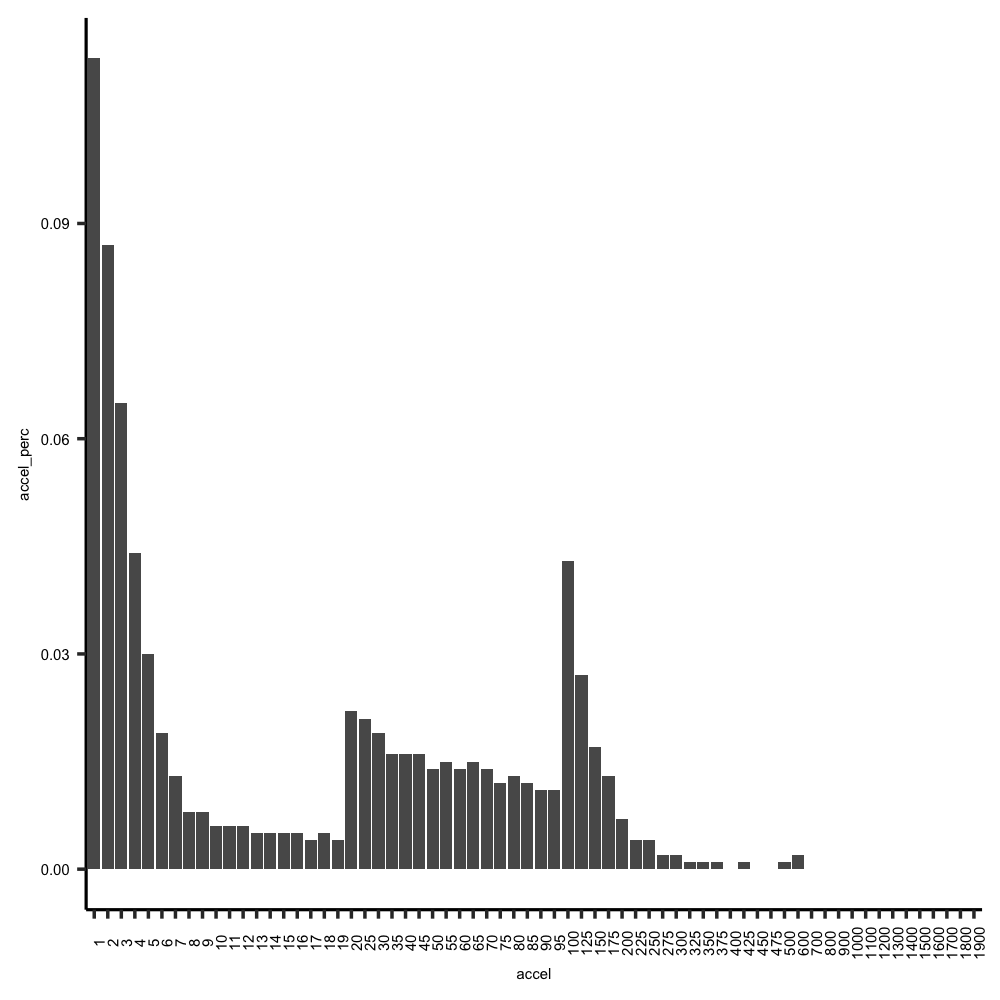
\includegraphics[width=0.75\linewidth,height=0.35\textheight,]{fig1} 

}

\caption{Sample Accelerometry Distribution}\label{fig:unnamed-chunk-4}
\end{figure}

\hypertarget{correlation-between-accelerometry-and-activity}{%
\subsubsection{Correlation Between Accelerometry and
Activity}\label{correlation-between-accelerometry-and-activity}}

As the intensity of activity is positively correlated to acceleration,
these 3 ranges of acceleration can be related to low, moderate and high
intensity activities respectively. By summing up all the fractions in
each range, the total fraction depicted the percentage of acceleration
triggered by the different kinds of activities. For example, the total
fraction of acceleration from 1 to 19 milli-gravities is proportional to
the amount of low-intensity activity. In following analysis, sum of
acceleration fractions would be taken as the value of certain activity
amount directly. Table 1 shows the map between acceleration and activity
groups.

\begin{table}

\caption{\label{tab:unnamed-chunk-5}Map of Acceleration and Activity Group}
\centering
\begin{tabular}[t]{cc}
\toprule
acceleration & activity\\
\midrule
1 - 19 milli-gravities & low-intensity activity\\
20 - 95 milli-gravities & mid-intensity activity\\
100 - 1900 milli-gravities & high-intensity activity\\
1 - 1900 milli-gravities & total activity\\
\bottomrule
\end{tabular}
\end{table}

\hypertarget{bivariate-analysis-activity-amount-vs.-medical-conditions}{%
\subsubsection{Bivariate Analysis: Activity Amount vs.~Medical
Conditions}\label{bivariate-analysis-activity-amount-vs.-medical-conditions}}

The Summary Data contained multiple variables indicating users' sleep,
psychological and medical conditions. For example,
\emph{overall\_health\_rating} taking values of \emph{Excellent},
\emph{Good}, \emph{Fair}, \emph{Poor}, \emph{Do not know} and
\emph{Prefer not to answer} indicated the overall health condition of a
user. Figure 2 is the box plot of activity amount grouped by
\emph{overall\_health\_rating}.

\begin{figure}[h]

{\centering 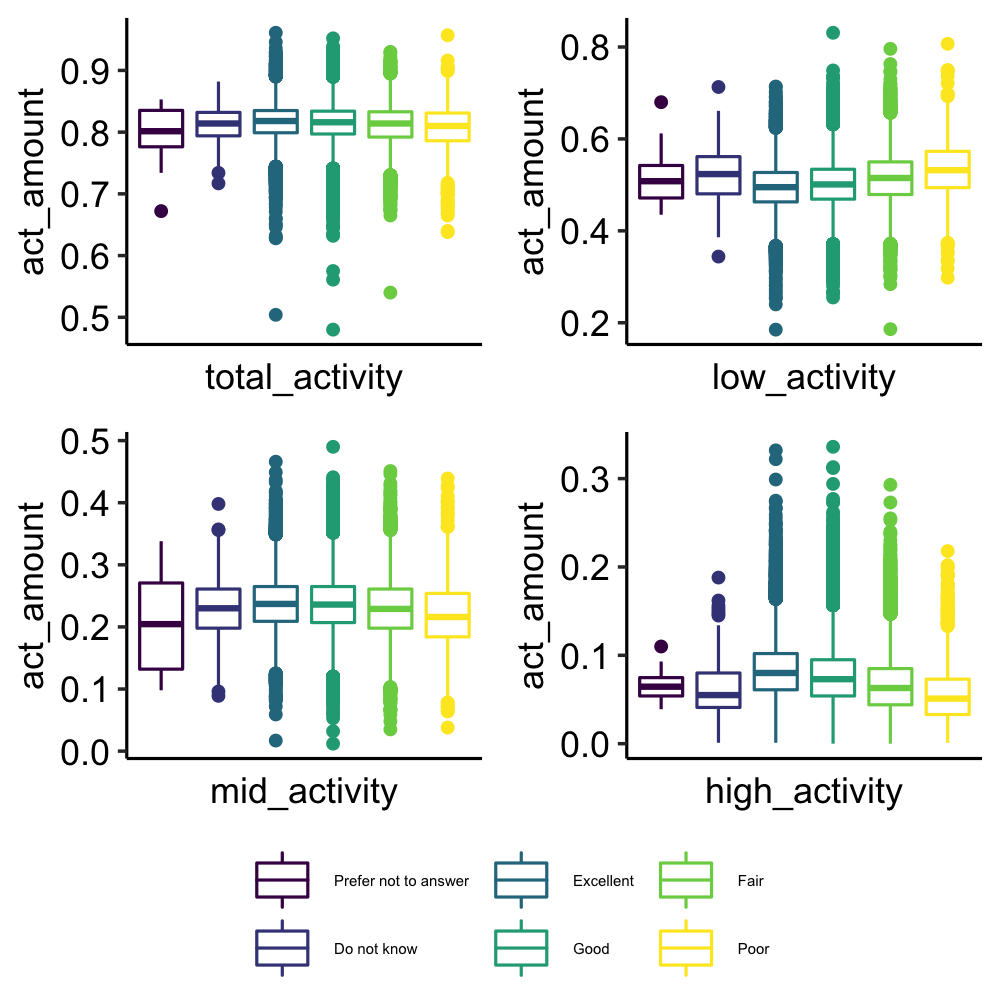
\includegraphics[width=0.7\linewidth,height=0.45\textheight,]{fig2} 

}

\caption{Box Plot of Activity Amount Group by Overall Health Rating}\label{fig:unnamed-chunk-6}
\end{figure}

In the subplot of high-intensity activity, the distributions of activity
amount for \emph{Excellent}, \emph{Good}, \emph{Fair} and \emph{Poor}
users had significant differences. The health ratings were positively
correlated to the amount of high-intensity activity. Similar patterns
can also be found in other medical variables.

\hypertarget{significance-validation}{%
\subsubsection{Significance Validation}\label{significance-validation}}

According to Central Limit Theorem, mean of activity amount for users
with a certain medical condition approximates a normal distribution.
Thus the differences between the mean of activity amount among users
with multiple medical conditions should also approximate a normal
distribution. Taking the minimal p-value for difference greater or less
than 0 as the final statistics, we were able to validate whether
activity amount can distinguish medical condition effectively.\\
\[
p.value = min\{p.value(mean~~difference > 0),~~p.value(mean~~difference < 0)\}
\]

Figure 3 showed the approximated normal distribution density plot for
the mean difference of high activity amount between users with
\emph{overall\_health\_rating} as \emph{Excellent} and \emph{Poor}. The
final p-value was 0, which meant the high activity amount was
significant to distinguish between users with ``best'' and ``worst''
health ratings.

\begin{figure}[h]

{\centering 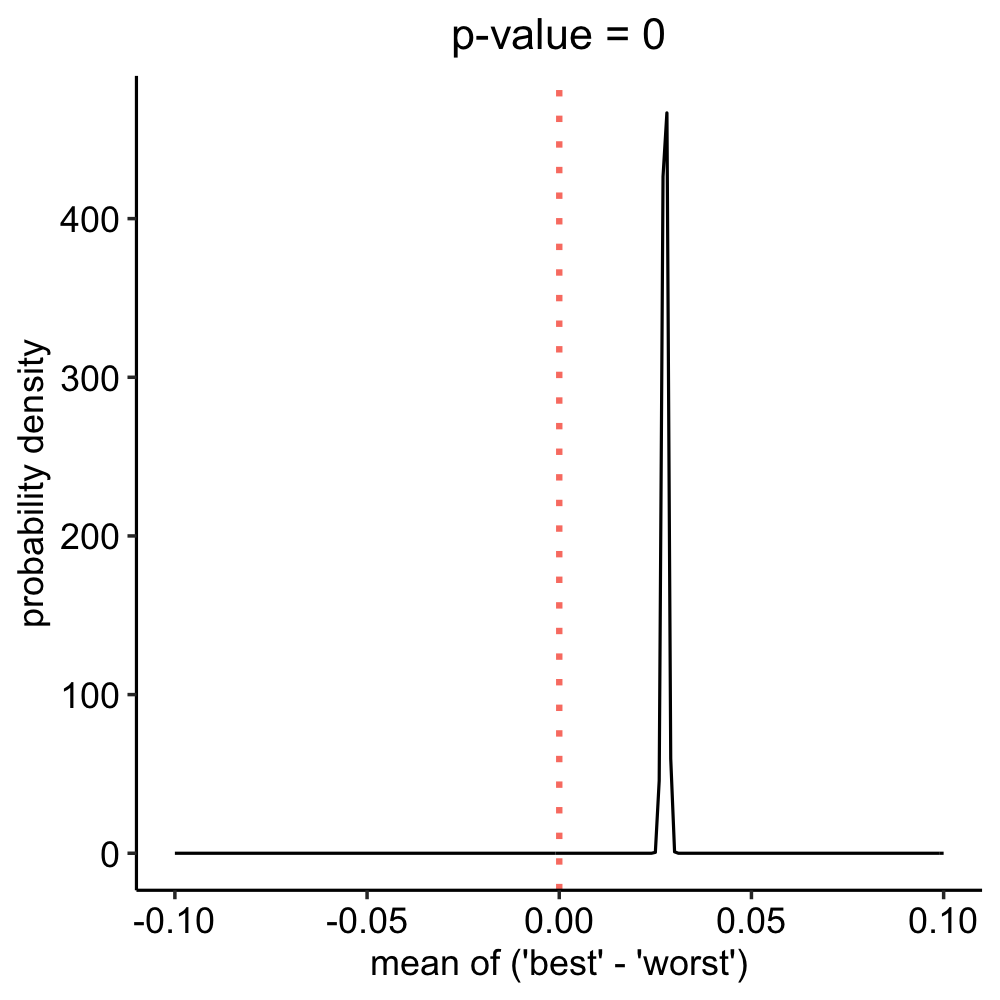
\includegraphics[width=0.65\linewidth,height=0.45\textheight,]{fig3} 

}

\caption{Normal Distribution Approximation for Mean of High Activity Amount Difference Between Excellent and Poor}\label{fig:unnamed-chunk-7}
\end{figure}

Taking a series of medical variables and conducting the significance
validation generated Table 2. It was obvious to see activity amount
worked effectively to distinguish the differences for a considerable
number of combinations in medical conditions.

\begin{longtable}[t]{>{\centering\arraybackslash}p{2cm}cccc}
\caption{\label{tab:unnamed-chunk-8}Significance Validation of Activity Amount Differences Between Medical Conditions}\\
\toprule
activity & medical.variable & Condition.1 & Condition.2 & p.value\\
\midrule
high & nap during day & Never/rarely & Usually & 0.0000\\
mid & nap during day & Never/rarely & Usually & 0.0000\\
low & nap during day & Never/rarely & Usually & 0.0000\\
high & neuroticism score & 0 & 11 & 0.0256\\
mid & neuroticism score & 0 & 11 & 0.1130\\
\addlinespace
low & neuroticism score & 0 & 11 & 0.0111\\
high & overall health rating & Excellent & Poor & 0.0000\\
mid & overall health rating & Excellent & Poor & 0.0000\\
low & overall health rating & Excellent & Poor & 0.0000\\
high & sleep duration & 18 & -3 & 0.0256\\
\addlinespace
mid & sleep duration & 18 & -3 & 0.3628\\
low & sleep duration & 18 & -3 & 0.0073\\
high & sleeping too much & No & Yes & 0.0000\\
mid & sleeping too much & No & Yes & 0.0000\\
low & sleeping too much & No & Yes & 0.0000\\
\addlinespace
high & sleeplessness insomnia & Never/rarely & Usually & 0.0000\\
mid & sleeplessness insomnia & Never/rarely & Usually & 0.0000\\
low & sleeplessness insomnia & Never/rarely & Usually & 0.0000\\
high & snoring & No & Yes & 0.0000\\
mid & snoring & No & Yes & 0.0000\\
\addlinespace
low & snoring & No & Yes & 0.0000\\
high & trouble falling asleep & No & Yes & 0.0272\\
mid & trouble falling asleep & No & Yes & 0.0116\\
low & trouble falling asleep & No & Yes & 0.0008\\
\bottomrule
\end{longtable}

\bibliographystyle{agsm}
\bibliography{bibliography.bib}


\end{document}
